% !TeX root = ../main-english.tex
% !TeX spellcheck = en-US
% !TeX encoding = utf8
% -*- coding:utf-8 mod:LaTeX -*-

%This smart spell only works if no changes have been made to the chapter
%using the options proposed in preambel/chapterheads.tex.
\renewcommand*\dictumwidth{0.5\linewidth}
\setchapterpreamble[o]{%
	\dictum[John Claerbout, rephrased by Buckheit \& Donoho]{An article about computational science in a scientific publication is not the scholarship itself, it is merely advertising of the scholarship. The actual scholarship is the complete software development environment and the complete set of instructions which generated the figures.}
}

\chapter{Introduction}
\label{chap:k1}

In natural settings, value-based decisions under risk often have to be made without visual presence of competing alternatives.
Do I commit to buying the red bicycle in the store I'm currently in, or should I return to the previous bike shop and pick the blue one?
Do I want to rent the flat I viewed last Sunday, or the apartment I saw on Tuesday?
In such situations, relevant properties of alternative options such as their subjective value have to be encoded, held in working memory through a maintenance (or ``delay'') period, and retrieved in order to form a categorical choice.\\
To understand the neural processes underlying behavior in these situations, the neural activity in the delay period and how it might represent or maintain relevant properties were a focus of research in the last decades.
Although several popular theories emerged over time and were either refuted or refined, and the field has progressed from studying spiking activity in single cells to computationally elaborate models of spatially and temporally distributed activity, a comprehensive understanding is yet lacking \citep{sreenivasan2019and}.
The main goal in the conception of this research project has been to make a contribution to the study of brain state dynamics in working memory, a recently emerging theory that reconceptualizes neural activity as a trajectory through a high-dimensional neural space.
To this end, I was given access to a pre-existing \gls{meg} dataset from human participants that played an experiment with a delayed decision making task, acquired by \citet{kaiser}, the \textit{memento} dataset.\\
This research endeavor posed several challenges.
One lay in acquiring the relevant information to work productively and confidently with this dataset.
Data was captured at the Clinic for Neurology at the Otto-von-Guericke University Magdeburg, an institution to which I did not have access or first-hand knowledge about.
The original lead investigators of the project had switched their focus to other projects by the time I started working with it, and both had left their research positions by the time I finished.
Obtaining their first-hand knowledge was thus impeded not merely by fading memory over time, but also as their progression to other projects and out of academia naturally limited contact.
While the dataset had been processed extensively already, the data was in an idiosyncratic organization, many existing analyses were in an interim state, and the project, excluding raw and processed data, was a collection totaling 20.761 files.
Thus, a prerequisite of my analyses was to prepare the dataset such that it became usable for me, and ideally also to future other researchers that were not involved in its acquisition or processing.\\
A different challenge lay in the processing setup.
The data were acquired and partially analyzed on infrastructure of the University of Magdeburg.
After a change of affiliations, storage and further analyses were moved to the computational cluster of the \gls{HHU}.
My own analyses, finally, were done on computational infrastructure at the Institute of Neuroscience and Medicine at the \gls{FZJ}.
Typically, changes of computational infrastructure are detrimental to the utility of the processing and analysis scripts.
Thus, an explicit aim of all processing was portability, such that research outcomes yielded on \gls{FZJ} infrastructure were readily usable on servers at the \gls{HHU} or elsewhere.\\
Finally, the to-be-conducted analyses were highly exploratory.
Although the dataset had not been published before, a large amount of analyses had already been conducted.
But with the exception of a poster presentation on preliminary decoding results \citep{kaiserposter}, all analyses yielded null results and remained unpublished.
Thus, in an attempt to extend previous analyses and search for remaining insights in the data with novel methodology, I set out to conduct analysis rooted in functional alignment and dimensionality reduction that have yet rarely been used on \gls{meg} data.
Maintaining routines for reproducibility and reusability, however, is not trivial when the analyses are not mapped out entirely and the necessary software for the analyses is in flux.
Keeping all analyses transparent, self-descriptive to others, and reproducible became a guiding principle.\\
Although the challenges I outlined above shaped the course of the project and gave way to productive projects to solve them, they are by no means uncommon in scientific endeavors.
Science is incremental and its outcomes go beyond journal articles -- code, data, results, or tools of previous finished or unfinished projects are reused or extended in later activities \citep{mons2018data}, and the people who start and finish a project are not necessarily the same \citep{puce2017review}.
Science is also increasingly collaborative and spatially distributed \citep{csomos2020exploring}.
Benefiting from differential expertise of several collaborators requires mutual understanding of a project and its components.
But the relevant research data management skills are not commonly part of research training curricula \citep{grisham2016proposed}. %, and publication practices that favor static PDFs of articles instead of the building blocks of the underlying science fail to incentivize the curation of well documented project directories (CITE).
Nevertheless, over several decades already, data shared across institutions or even openly has been a corner stone of neuroscientific progress \citep[e.g.,][]{ferguson2014big, niso2016omega}, and this trend is increasing \citep{gorgolewski2016practical}.
A common challenge is thus to keep projects in such a state that they can be understood without the expertise of their original authors \citep{puce2017review}.
This makes technical and organizational elements of scientific practice, such as \gls{rdm} and research software engineering, a fundamental prerequisite.
Going sequentially through the different challenges and solutions to conducting reproducible brain state analyses, this thesis summarizes my conjunct work on research data management solutions, research software engineering practices, and their application in a scientific project that spanned several institutions and generations of researchers.\\
To lay the foundations for this, the remainder of the introduction establishes a number of prerequisites.
The first section \ref{chap:k1-brain} outlines a brief overview of the literature in the field of working memory maintenance, and deduces the choice of analyses methods for dimensionality reduction for the study of brain states in Chapter \ref{chap:k4}.
Afterwards, section \ref{chap:k1-rdm} introduces the topic of research data management, and highlights central concepts and tools that will be a focus in the upcoming chapters \ref{chap:k2} and \ref{chap:k3}.
As I will lay out in this section and in upcoming chapters, \gls{rdm} is a foundational element within good scientific practice, and an important prerequisite for computational neuroscience.

\section{Brain state spaces}
\label{chap:k1-brain}
%This is an introduction into brain states and functional alignment

The concept of \textit{brain states}, global neural activity patterns that are associated with distinct cognitive processes or behavioral states, has emerged in the study of various brain functions, from sleep \citep{lee2012neuromodulation}, to motor processes \citep{pfurtscheller2008short}, or functional connectivity \citep{finn2017can}.
Over the course of the last decades, it also emerged in the study of working memory. \\
Early neuroimaging and electrophysiology studies suggested persistent neural activity (``spiking'') in specific brain areas during delay periods as a mechanism of working memory maintenance \citep{goldman1995cellular}.
Sustained, above-baseline activity that starts during a sample presentation, lasts through the memory delay, and returns to base line activity after a response were found in prefrontal regions in human \citep[e.g.,][]{courtney1997transient} and non-human primates \citep[e.g.,][]{fuster1971neuron, funahashi1989mnemonic, miller1996neural}.
And single-cell recordings from the prefrontal cortex in monkeys unveiled that individual neurons display activity that is selective to specific task-relevant aspects, such as task rules, spatial location, or stimulus features \citep{white1999rule, wallis2001single}, suggesting the existence of neurons that uphold working memory content with a fixed selectivity for certain properties.
Others have pointed out, however, that persistent spiking in prefrontal areas could reflect a variety of other different processes, including decision making \citep{curtis2010beyond} or anticipation of the probe \citep{nobre2011attention}, that the high metabolic costs of action potentials is too energetically expensive to hold information in a spiking form \citep{attwell2001energy}, and that distractor tasks are able to remove the persistent activity without an impact on later retrieval, questioning its role in working memory maintenance \citep{larocque2013decoding, lewis2015neural}.\\
The idea of neural selectivity to specific task-aspects was refined in the adaptive coding framework \citep{duncan2001adaptive}:
Instead of a persistent, fixed selectivity, it postulates that neural responses are temporarily tuned to the particular task. This theory was able to explain how a recording of spiking activity in the same group of neurons relates to object information in one task but a location distinction in the next task \citep{duncan2001adaptive}.
\citet{mongillo2008synaptic} proposed a highly influential theory according to which short-term neural plasticity changes are the underlying mechanism of working memory maintenance.
According to it, working memory maintenance is established via increased residual calcium levels at the presynaptic terminals of neurons, which causes a short-term synaptic facilitation, akin to synaptic weights that link neurons coding for a working memory item.
With this facilitation, the memory can be transiently held for about 1s without enhanced spiking activity in a network of neurons.
Building up on this theory,  \citet{stokes2015activity} proposed the dynamic coding framework, in which working memory is mediated by rapid transitions in such ``activity silent'' neural states.
While these states mediate flexible, context-dependent processing they do not emerge as constant activity and rather as ``hidden states'', appearing as altered response sensitivities of neural networks, established via short-term and long-term synaptic plasticity and temporal functional connectivity changes that influence the response to stimuli.
An explanation why spiking activity is nevertheless found during delay periods comes from findings that a task-irrelevant read-out or ``ping'' signal is able to reactivate the neural assembly \citep{trubutschek2017theory}.
This raises the possibility that previous findings of neuronal spiking might have been similar readouts from an activity silent population after task-irrelevant non-specific inputs \citep{wolff2017dynamic}.
Alternatively, \citet{fiebig2017spiking} hypothesized that occasional spiking of memory-encoding neurons is needed to refresh the activity-silent states.\\
The idea that distributed representations that selectively favor information relevant to the current task emerge on the level of neural populations was central in other theories as well.
\citet{rigotti2013importance} proposed the concept of mixed selectivity, in which information is distributed across neurons through non-linear and high-dimensional representations even when it is not observable in individual cells.
The rise of multivariate methods such as decoding analyses gave way to thorough investigations of distributed neural patterns.
\citet{king2014characterizing} formalized this with the temporal generalization method.
In this method, several classifiers are trained on different time slices of training data each, and tested on all available times in the test data, thus revealing whether the neural code is stable or dynamically evolving.
Interestingly, studies decoding working memory content found that decodable patterns can be non-stationary.
\citet{meyers2008dynamic} decoded object categories from electrophysiological data, and yielded worse decoding the more temporally distant training and testing times slices were apart.
\citet{stokes2013dynamic} used temporal cross-correlation analyses to show that population responses in the prefrontal cortex evolve during a memory delay.
These representations of task-relevant stimulus information in temporarily and spatially distributed activity across neurons were termed dynamic population coding \citep{sreenivasan2014revisiting} (see Figure \ref{fig:dynamiccoding}).\\
The theory that cognitive processes evolve through different brain states as dynamic neural trajectories is line with non-stable representations \citep{buonomano2009state}.
These trajectories emerge by conceptualizing neural responses as vectors in an N-dimensional space that evolves over time:
The axes of the high-dimensional space correspond to measurements, such as raw or transformed data from M/EEG sensors or \gls{fMRI} voxels.
Each time point in the acquisition becomes a point in the high-dimensional space spanned by all sensors, determined by the measurement in each sensor, such as activation strength.
In geometric terms, this point is an N-dimensional vector.
Neural trajectories emerge by tracing the activity on these axes over multiple time points.
Common or distinct brain states could then become evident as converging or diverging trajectories (see Figure \ref{fig:trajectories}).

\begin{figure}[H]
	\begin{subfigure}{\textwidth}
		\centering
		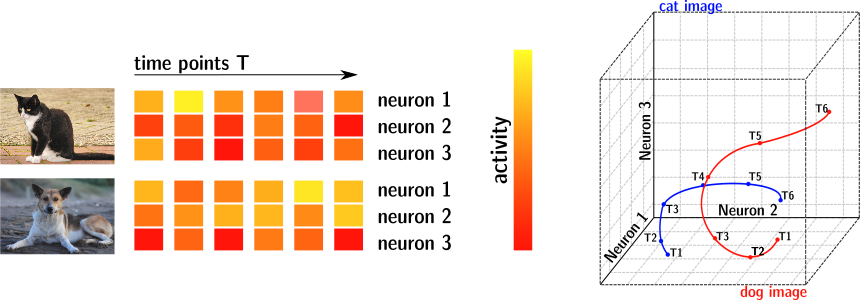
\includegraphics[width=0.8\textwidth]{memento/dynamic_coding.png}
		\caption {The dynamic coding framework}
		\label{fig:dynamiccoding}
	\end{subfigure}
	\hfill¸
	\begin{subfigure}{\textwidth}
		\centering
		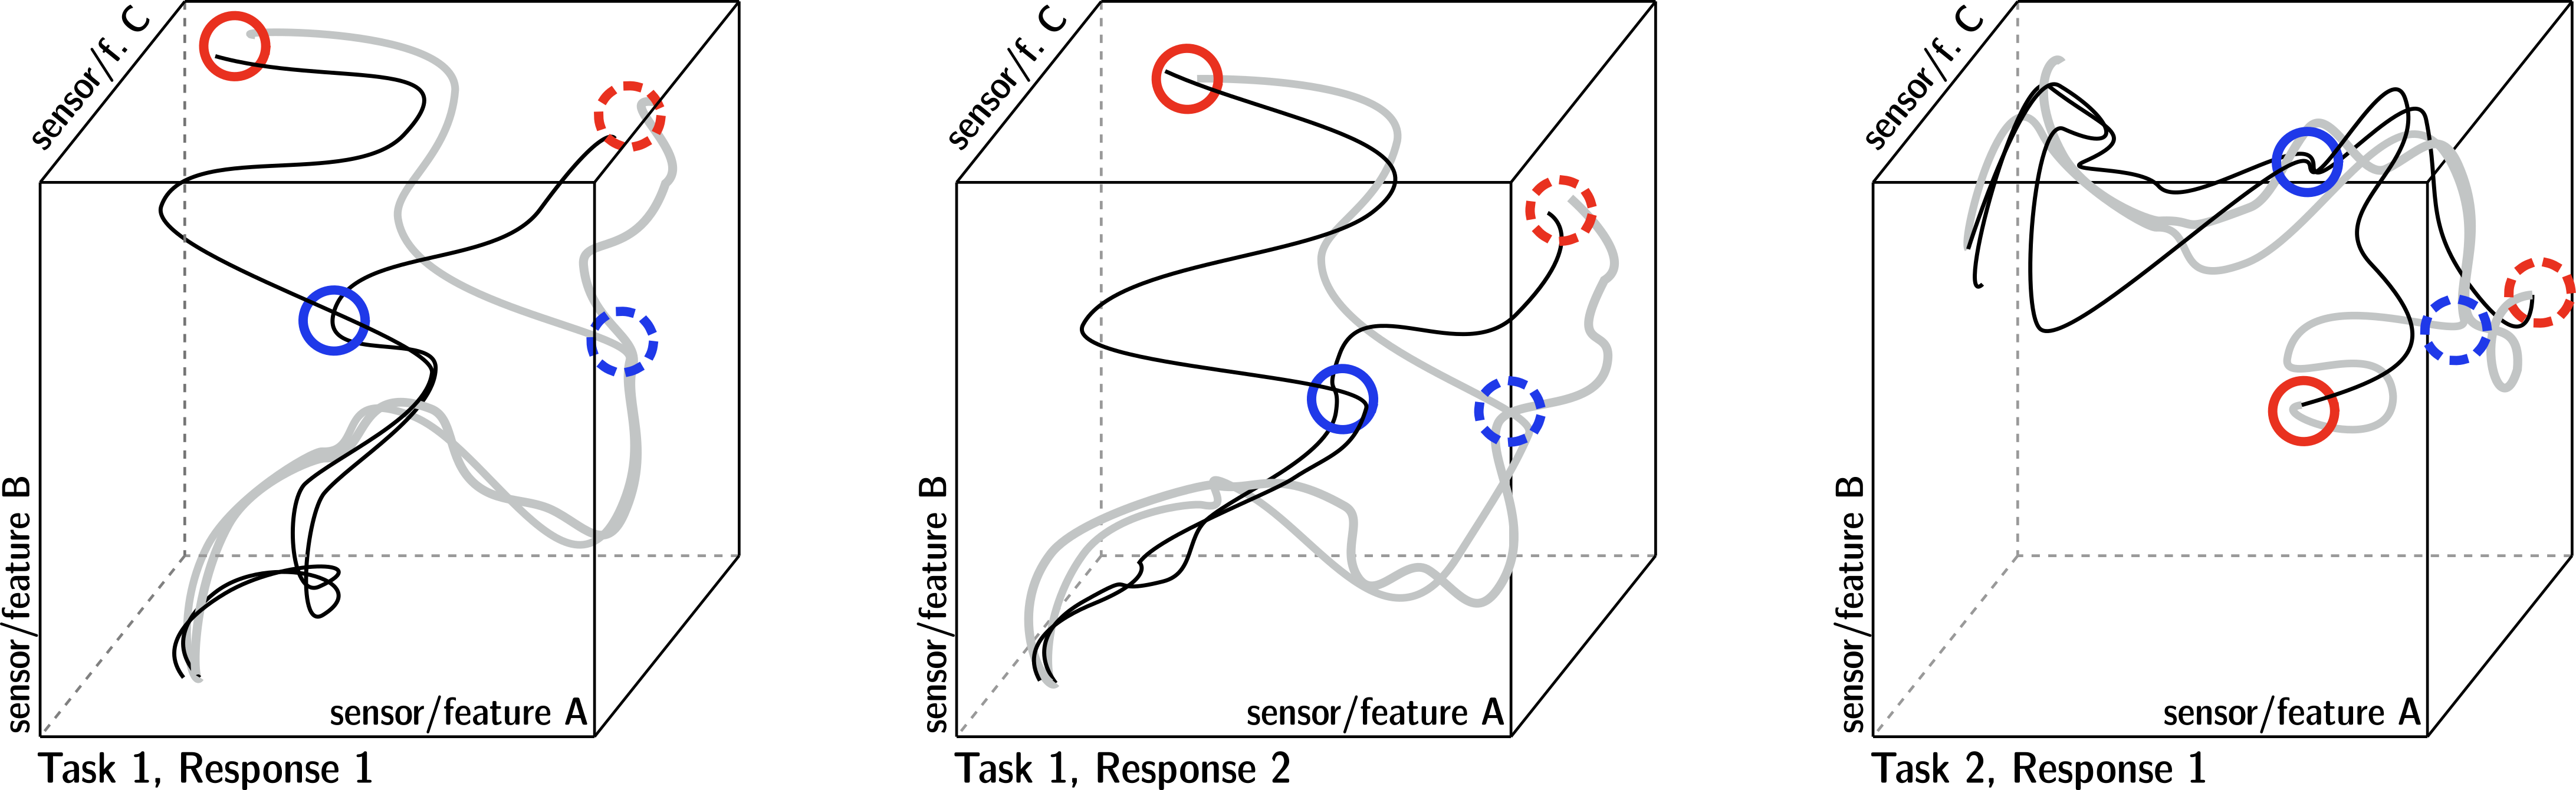
\includegraphics[width=0.8\textwidth]{memento/neural_trajectories_redone.png}
		\caption{Idealized neural trajectories through state-spaces}
		\label{fig:trajectories}
	\end{subfigure}
	\caption[Dynamic coding and neural trajectories in the study of brain states]{A schematic illustration of dynamic coding in neural populations as trajectories through high dimensional spaces. The left side of a) depicts a population of three neurons (squares), and their activity (color) over six time points time in response to two visual stimuli. The neural code in this population is not stationary, but dynamic: Each stimulus evokes a distinct response, but within this response, each time point has a different pattern of neural activity, too. By conceptualizing activity patterns over time as vectors, these patterns can be visualized in a multi-dimensional space (right). This space has as many dimensions as there are measurement sites (e.g., neurons, sensors, voxels, or electrodes). Dynamic population codes create trajectories through this space. Adapted from \citet[][Fig. 2]{meyers2018dynamic}. b) shows an idealized illustration of neural trajectories in different states for two decision alternatives (blue) and two response alternatives (red), for two tasks in a delayed-response-mapping paradigm. Assigning meaning to the axes of the state-space may yield insights about brain states in different experiment conditions. Adapted from Jocham, Krauel, Hanke (unpublished).}
	\label{fig:brainstates}
\end{figure}


To bridge the gap to theories of activity silent states, the neural responses that form dynamic trajectories are not solely determined by external stimuli, but also internal state changes of the network, such as the strength of synaptic connections, or excitatory or inhibitory influences from other networks \citep{buonomano2009state}.
Distinct neural states were often hypothesized to reflect steps in mental processing \citep[e.g.,][]{seidemann1996simultaneously}.
\citet{muhle2021hierarchy}, for example, proposed a hierarchy of functional states in working memory, with items relevant for a pending decision in the most active state, and items relevant only for later use in latent states.
But studies were also able to extract external stimulus information from the trajectories of transient states, for example odors \citep{mazor2005transient}.
The study of these neural states and their transition has emerged as its own field, employing multivariate methods such as decoding across neural populations, hidden Markov models (HMMs) \citep{rainer2000neural} to model ensemble activity as a sequence of constantly shifting neural states \citep{vidaurre2016spectrally}, or functional alignment \citep{haxby2011common} to find common representations across idiosyncratic neural responses.\\
In parallel, dimensionality-reduction gained popularity in the analysis of neural population data \citep{cunningham2014dimensionality}.
Though partially rooted in attempts to make analyses computationally feasible, a central underlying justification of dimensionality reduction approaches is that the measured neural activity is too complex compared with the few relevant task or stimulus aspects that require encoding, and that the neural signal of interest must be embedded in a subspace of the high-dimensional neural space.
\citet{santhanam2009factor} for example employed a decoding approach based on factor-analysis to reduce noise in high-dimensional neural recordings to improve the performance of neural prostheses, which otherwise suffered from the neural variability introduced by changes in attentional state or wakefulness.
The motor signal of interest thus lay embedded in a high-dimensional space containing variability from unrelated cognitive sources, and identifying this subspace improved the study of the signal of interest.
Fittingly, the term ``effective dimensionality'' of population activity emerged in the literature to identify shared components of collective dynamics that reflect task variables \citep{jazayeri2021interpreting}.
Investigations of dynamic or stable population codes for working memory have been done in conjunction with dimensionality reduction methods, too, and yielded interesting observations.
\citet{murray2017stable} used \gls{pca} on electrophysiology recordings acquired from primate prefrontal cortex during a working memory task.
They found a lower-dimensional subspace in the high-dimensional state space in which stimulus representations were stable across the cue and delay epochs.
\citet{machens2010functional} likewise used \gls{pca} in a working memory task where non-human primates compared the frequency of two vibrations to identify a 6-dimensional subspace in which this tactile stimulus information is represented.\\
%Of relevance for these findings could also be the neural manifold hypothesis \citet{gallego2017neural}.
%In this hypothesis, behavior is controlled by neural \textit{modes}, patterns of neural population covariance.
%The high-dimensional neural space is confined into a lower dimensional ``manifold'' spanned by these neural modes, and dimensionality reduction methods could allow the study of neural population dynamics within them.
%Importantly, they further showed that the low dimensional spaces remained stable over multiple years when aligning these manifolds \citep{gallego2020long}.\\
Studying working memory maintenance using dimensionality reduction methods and the concept of neural trajectories through a state-space is thus a promising approach for new insights.
It re-conceptualizes neural function from averaged spiking activity that aims to draw conclusions about the brain area of a cognitive process, to dynamics in multi-dimensional spaces that might bear the potential to draw conclusions about the lower-dimensional components our cognition is build up on.
The path from data acquisition or raw data to such a data analysis is, however, more complex than the method section of the final paper makes it appear.
Before this thesis continues with the analyses of neural trajectories in working memory, the upcoming two chapters and the remainder of the introduction are dedicated to concepts and projects around \gls{rdm} that were ultimately relevant pillars of the project.
%\citep{vidaurre2016spectrally} investigated brain state time courses identified by a HMM-based approach by their spectral properties.

%In voluntary movement performing, the M1 neural population undergoes a state of desynchronisation followed by a synchronisation period. These are usually referred to as event-related desynchronisation (ERD) and event-related synchronisation (ERS). from https://www.sciencedirect.com/science/article/pii/S1053811915010691

%Drawing insights from this partial overview of the literature, methods to study working memory have shifted from traditional evoked potentials to computationally intensive processing.
%The field has progressed from studying spiking activity in single cells to an implicit consensus that the neural representation of working memory during maintenance is high-dimensional or embedded in a high-dimensional space, time-varying, and spatiotemporal distributed.
%But despite the wealth of theories and methodological approaches, the field has not yet converged on a full understanding of working memory.
%Recent reviews have begun to point out where findings and standard views fall short to yet explain the mechanisms underpinning working memory \citep{nobre2022opening}, or highlight the inconsistencies in results across studies \citep{pavlov2022oscillatory}.
%While studies traditionally focused on the involvement of prefrontal areas due to its involvement in executive control \citep[e.g.,][]{fuster1971neuron, funahashi1989mnemonic, miller1996neural}, many other brain areas have been shown to represent working memory items, too.
%In a recent review, \citet{sreenivasan2019and} summarized how single-cell measurements, MEEG, and \gls{fMRI} acquisitions have found increased activity during working memory maintenance throughout the cortex and even some subcortical areas.
%\citet{d2007cognitive} described working memory as an emergent property of functional interactions prefrontal areas and the rest of the brain as opposed to being localized to a single brain region.
%And while an often proposed mechanism for the coordination of temporal and spatial population codes are brain oscillations in specific frequency bands \citet[e.g.,][]{roux2014working}, %for example concluded that gamma and alpha band oscillations of groups of neurons are generically involved in the maintenance of sensory-spatial working memory items.
%a recent systematic review by \citet{pavlov2022oscillatory} highlighted a prominent lack of agreement across results in experimental studies that reported observations of brain oscillations in working memory tasks.\\
%%Decoding approaches can find multiple different working memory items simultaneously in the same neural population \citep{rigotti2013importance}, and in various brain regions \citep{curtis2010beyond}.
%In light of variable and even conflicting findings, \citet{nobre2022opening} called for sustained open-mindedness and creativity in researching working memory in a recent reflective piece.
%In this exploratory spirit, I conducted the simulations and analyses that will be described in this chapter.
%They connect to the works of \citet{murray2017stable}, \citet{machens2010functional}, \citet{rigotti2013importance} and others who employed dimensionality reduction methods perform statistical decomposition in a high dimensional ``native neural space'' to
%project the axes of a task space into subspaces of the native neural space (see Figure \ref{fig:trajectories}).
%They do not confine the neural signal to a specific brain area, but attempt to find neural signatures of decision-relevant working memory items across the cortex.
%Central to the analyses is the attempt to use a method for functional alignment and dimensionality reduction on \gls{meg} data.



%\begin{figure}
%	\centering
%	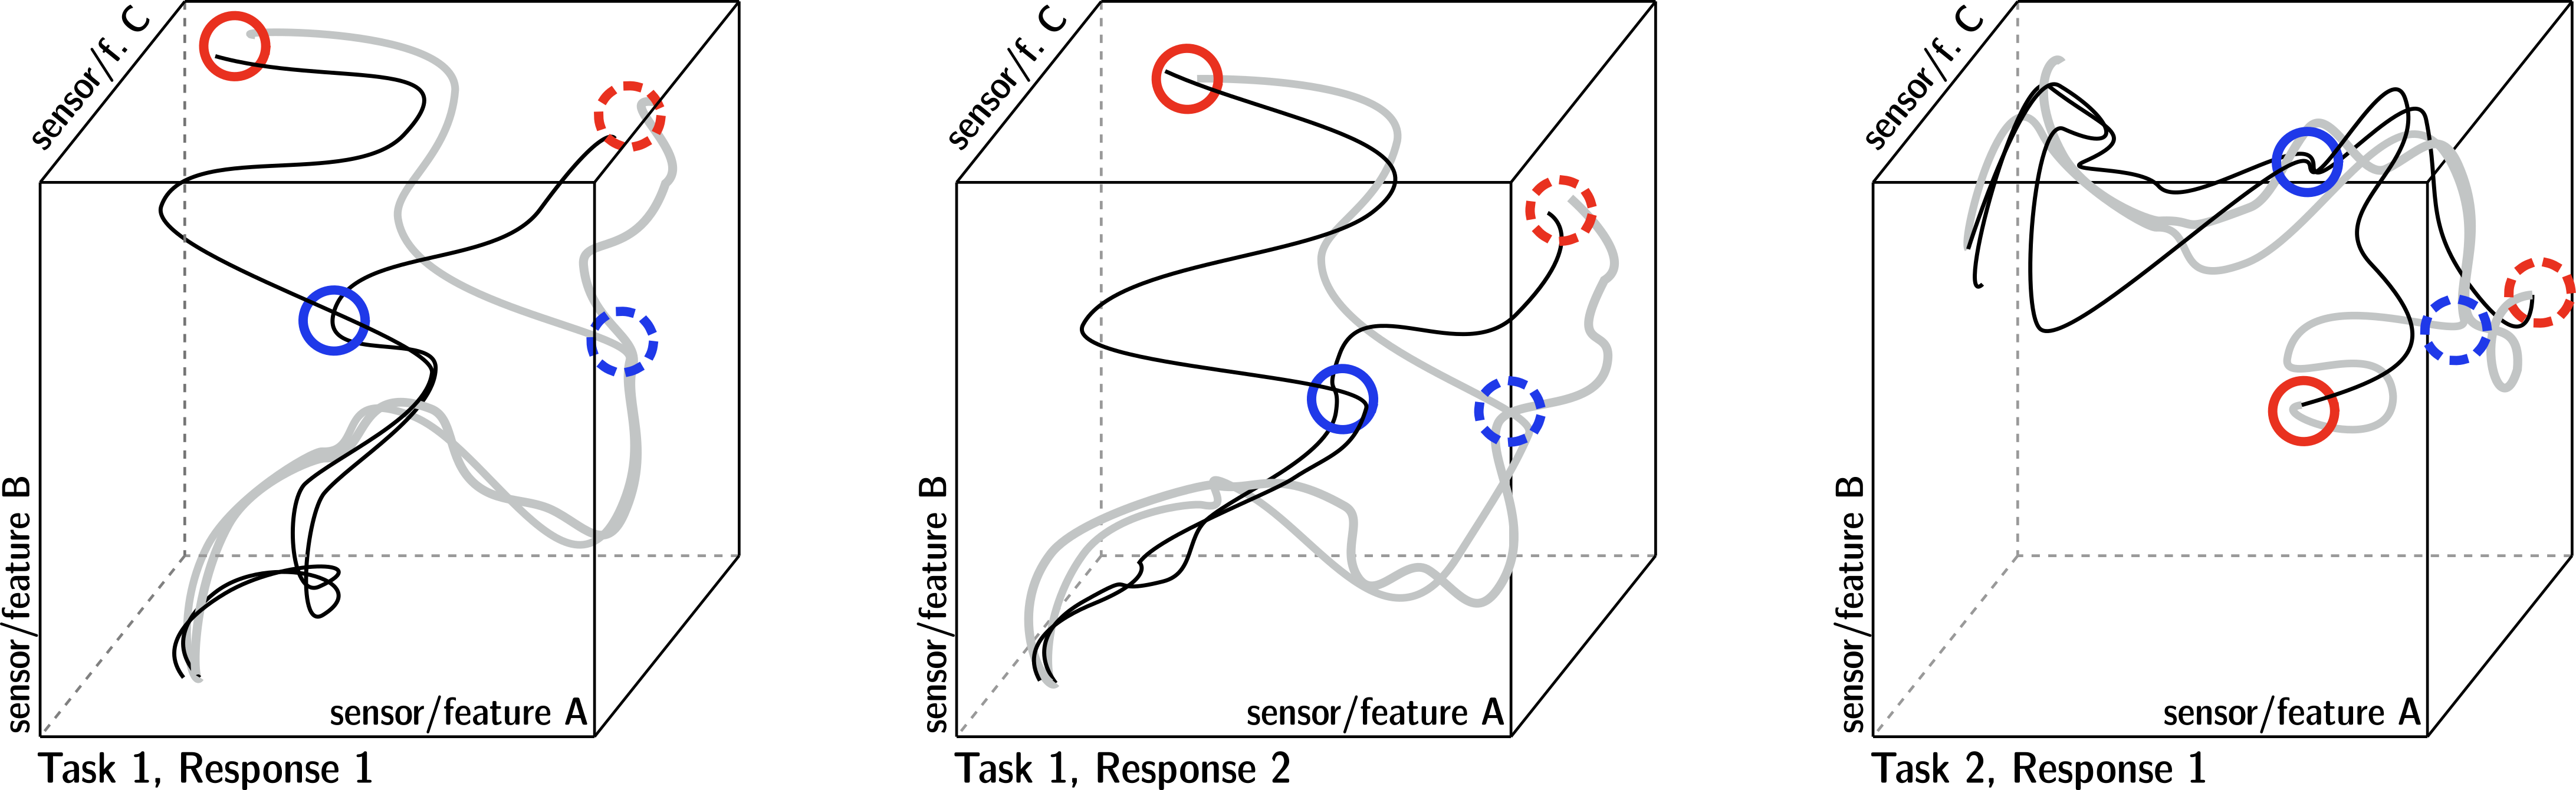
\includegraphics[width=0.5\textwidth]{memento/neural_trajectories_redone.png}
%	\caption[Neural trajectories through state-spaces]{An schematic illustration of neural trajectories through a state-space for two decision alternatives (blue) and two response alternatives (red), for two tasks in a delayed-response-mapping paradigm. Assigning meaning to the axes of the state-space may yield insights about brain states in different experiment conditions. Adapted from Jocham, Krauel, Hanke (unpublished)}
%	\label{fig:trajectories}
%\end{figure}




%The decoding approach, generally speaking, works by identifying patterns that correspond to the experimental task or stimulus in population signals with machine-learning classifiers.


\section{Research data management}
\label{chap:k1-rdm}
%This is an introduction on the importance of research data management for reproducible science

A foundation of scientific insight lies in research data management.
Research data encompasses everything that is produced in the life span of a research project.
From raw data acquisitions, preprocessed or otherwise standardized datasets, to software, analysis scripts, results, figures, compiled reports, and other final or intermediate research outcomes.
To disambiguate the term ``research data'' from the smaller-scoped meaning of ``data'' in colloquial language (the outcome of a data acquisition in an experiment), it is also referred to as ``research objects``, and, in case it exists in purely electronic form, as ``digital research objects'' \citep{bechhofer2010research}. \\
Typically, research objects have a much longer life span than the project that creates them.
Science is an incremental process that produces and builds up on more than just published journal articles \citep{mons2018data}, and code, data, results, or tools of previous finished or unfinished projects fuel new undertakings.
\gls{rdm} describes the handling of these research objects through their entire life cycle: from curation, use, publication and sharing, archiving to re-use or destruction (\cref{fig:rdm-lifecycle}).
Ultimately, it ensures that research objects are preserved to act as an evidence base for findings, and as a discoverable resource for further reuse.


\begin{figure}[H]
	\centering
	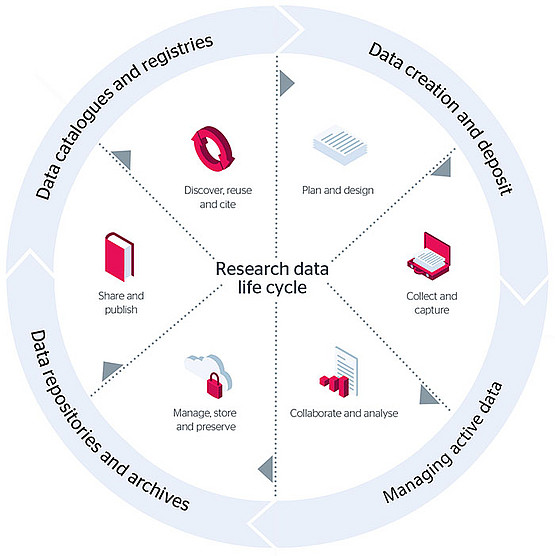
\includegraphics[width=.5\textwidth]{rdm-lifecycle-jisc.png}
	\caption[The life cycle of digital research objects]{The life cycle of digital research objects. License: JISC Research data management toolkit (\href{https://www.jisc.ac.uk/guides/rdm-toolkit}{www.jisc.ac.uk/guides/rdm-toolkit}), CC-BY-ND}
	\label{fig:rdm-lifecycle}
\end{figure}


\subsection{The FAIR guiding principles for scientific data management and stewardship}

Since their publication, the so-called \glsunset{FAIR}\gls{FAIR} principles \citep{wilkinson2016fair} have become guidelines for \gls{rdm} efforts for digital research objects.
They describe four measurable properties of research data that -- the better they are fulfilled -- serve the ultimate goal to improve the discoverability and reusability of data by machines and humans alike \citep{wilkinson2016fair}.
The \gls{FAIR}ness of data can be improved on each of the four related but separable major characteristics that are behind the \gls{FAIR} acronym (taken verbatim from Wilkinson et al.):

\begin{itemize}
	\item \textbf{F}indable: To be Findable, (meta)data  are assigned a globally unique and persistent identifier (F1); data are described with rich metadata (F2); metadata clearly and explicitly include the identifier of the data it describes (F3);  (meta)data are registered or indexed in a searchable resource (F4)
	\item \textbf{A}ccessible: To be Accessible, (meta)data are retrievable by their identifier using a standardized communications protocol (A1); the protocol is open, free, and universally implementable (A1.1); the protocol allows for an authentication and authorization procedure, where necessary (A1.2);  metadata are accessible, even when the data are no longer available (A2)
	\item \textbf{I}nteroperable:  To be Interoperable, (meta)data use a formal, accessible, shared, and broadly applicable language for knowledge representation (I1); (meta)data use vocabularies that follow FAIR principles (I2); (meta)data include qualified references to other (meta)data (I3);
	\item \textbf{R}eusable: To be Reusable, meta(data) are richly described with a plurality of accurate and relevant attributes (R1); (meta)data are released with a clear and accessible data usage license (R1.1); (meta)data are associated with detailed provenance (R1.2); (meta)data meet domain-relevant community standards (R1.3)
\end{itemize}

A pivotal factor for the importance of the FAIR principles is the increasing digitization of research practice, and with it, a rapid growth in research data \citep{dfg}.
Innovation relies on the ability to integrate new and existing data, and where the amount of data to discover, understand, and consolidate requires automation, research objects themselves need to become self-descriptive.
For this, the term ``machine-actionable'' is central to the \gls{FAIR} principles.
It is used to describe an ideal state in which a digital object provides detailed information (metadata) to an autonomously-acting, computational data explorer in two possible contexts: For one, as metadata about the object (``What is it?''), and second, as metadata about its content (``How do I process it?'') \citep{wilkinson2016fair}.
Notably, the \gls{FAIR} principles do not suggest specific metadata standards, implementations, or technology choices.
They do highlight the importance of community-endorsed vocabularies, however, and advocate to either extend them if they do not yet include the attributes required for rich annotations, or create suitable new community-endorsed vocabularies. \\
The end state of FAIR \gls{rdm} for any digital research object is a high quality digital publication that facilitates and simplifies its discovery, evaluation, and reuse in downstream studies.
This reusability refers to the further use or utilization inside or outside its original research context, by the original author or different actors.
It is arguably the most important feature of a research object for various stakeholders: It can make research more efficient, foster collaborations, and speed up progress, and as it can reduce duplicate efforts it constitutes an economical benefit for funders as well as the public and industry \citep{nfdi2022data}.
Considering additional time spent, cost of redundant storage, licensing costs, research retraction, double funding, and missed potential for economic growth, the European Commission estimates that the cost of not having FAIR data lies between 10 and 26 billion euro per year \citep{eu2019FAIR}.
The largest position in their cost-benefit analysis is the time wasted by researchers when non-FAIR data takes more time to find, retrieve, clean, integrate, and peer review.
The remainder of this chapter will outline \gls{rdm} requirements and solutions in the field of neuroimaging that aim to increase reusability.
They will come into practice in the preparation of the dataset in Chapter \ref{chap:k4} as reusing previous findings has played a central part in this thesis as well.
But one aspect of reusability is reproducibility to establish trust, which is a more important side effect of good data management than a cursory reading of the \gls{FAIR} principles implies.
The topic of reproducibility will thus also be continued later, and it is central to Chapter \ref{chap:k3}.

% Internationally accepted standard
%The largest funding institution for the sciences and humanities and research in Germany, the \gls{grf}, states that access to data and software according the the FAIR principles are of comparable importance to science as access to publications \citep{dfg}





\subsection{Research data management in neuroimaging}
\label{chap:k1-rdm-2}

%\[
%\left[
%\begin{tabular}{@{\quad}m{.3\textwidth}@{\qquad}m{.6\textwidth}@{\quad}}
%	\includegraphics[width=.7\linewidth]{qr_pub_niso.png} &
%	\raggedright%
%	\textbf{Related publications} \par
%	The following section contains a subset of the work presented in our original publication \citet{NISO2022119623}.
	%
%\end{tabular}
%\right]
%\]


Neuroimaging data poses a number of additional challenges for research data management.
For one, the field is characterized by complex datasets.
They typically encompass different modalities (such as imaging, electro-physiological, and behavioral measurements), and often entail several recording sessions.
The \gls{BIDS} \citep{gorgolewski2016brain} is a community-endorsed standard for organizing and describing neuroimaging data, and is widely considered as a successful solution for data standardization in such datasets.
It defines common and modality specific schemes for file names and file organization, file formats, and metadata to accompany raw  or derived data, i.e., both original acquisitions as well as the outputs of common processing pipelines.
\gls{BIDS} has widespread and growing support for different neuroimaging modalities, and is made a common prerequisite by neuroscientific data portals such as OpenNeuro \citep{markiewicz2021openneuro} or processing tools such as BIDSApps \citep{gorgolewski2017bids} or fMRIprep \citep{esteban2019fmriprep}.
An example of the \textit{memento} \gls{meg} dataset, organized idiosyncratically or structured according to \gls{BIDS}, is shown in \cref{fig:BIDS}. \\
%BIDS
\begin{figure}[H]
	{\tiny
		\begin{minipage}{.49\textwidth}
			\begin{forest}
				pic dir tree,
				for tree={% kleiner Zeilenabstand
					s sep=0.02cm}
				[memento/
				[memento\_001/
				%		[Move\_correc\_SSS\_alignedinitial\_nonfitiso/
				%		[1\_memento\_001\_ml83-1\_mc\_transforminitial.fif, file]
				%		[2\_memento\_001\_ml83-1\_mc\_transforminitial.fif, file]
				%		[3\_memento\_001\_ml83-2\_mc\_transforminitial.fif, file]
				%		[data\_fix1.mat, file]
				%		[data\_fix\_ft1.mat, file]
				%		[data\_fix\_new1.mat, file]
				%		[data\_fix\_reduced1.mat, file]
				%		[delay\_photodiode\_subject\_long\_default\_realign\_only\_ICA1.mat, file]
				%		[memento\_results\_ICA\_newall\_alignedinitial228.mat, file]
				%		[memento\_results\_ICA\_newall\_alignedinitial461.mat, file]
				%		[memento\_results\_ICA\_newall\_alignedinitial511.mat, file]
				%		[num\_trials\_old\_ICA.mat, file]
				%		[resultfile\_probs-1.mat, file]
				%		[trial\_out\_ind.mat, file]
				%		]
				[Move\_correc\_SSS\_realigneddefault\_nonfittoiso/
				[1\_memento\_001\_ml83\_mc\_realigneddefault.fif, file]
				[2\_memento\_001\_ml83-1\_mc\_realigned\_default.fif, file]
				[3\_memento\_001\_ml83-1\_mc\_realigned\_default.fif, file]
				[memento\_results\_ICA228.mat, file]
				[memento\_results\_ICA455.mat, file]
				[memento\_results\_ICA461.mat, file]
				[memento\_results\_ICA511.mat, file]
				[memento\_results\_ICA\_newall228.mat, file]
				[memento\_results\_ICA\_newall455.mat, file]
				[memento\_results\_ICA\_newall461.mat, file]
				[memento\_results\_ICA\_newall511.mat, file]
				[mri\_aligned.mat, file]
				[num\_trials\_old\_ICA.mat, file]
				[outfile\_new\_all.mat, file]
				[resultfile\_new\_all.mat, file]
				[template\_grid.mat, file]
				[trial\_out\_ind.mat, file]
				]
				[Raw/
				[1\_memento\_001\_ml83.fif, file]
				[2\_memento\_001\_ml83-1.fif, file]
				[memento\_001\_ml83-2.fif, file]
				]
				]
				]
			\end{forest}
		\end{minipage}
		\quad
		\begin{minipage}{.49\textwidth}
			\begin{forest}
				pic dir tree,
				for tree={% kleiner Zeilenabstand
					s sep=0.02cm}
				[memento/
				[dataset\_description.json, file]
				[participants.json, file]
				[participants.tsv, file]
				[README, file]
				[sub-001/
				[meg/
				[sub-001\_acq-calibration\_meg.dat, file]
				[sub-001\_acq-crosstalk\_meg.fif, file]
				[sub-001\_coordsystem.json, file]
				[sub-001\_task-memento\_channels.tsv, file]
				[sub-001\_task-memento\_events.tsv, file]
				[sub-001\_task-memento\_log.tsv, file]
				[sub-001\_task-memento\_meg.json, file]
				[sub-001\_task-memento\_split-01\_meg.fif, file]
				[sub-001\_task-memento\_split-02\_meg.fif, file]
				[sub-001\_task-memento\_split-03\_meg.fif, file]
				]
				[sub-001\_scans.tsv, file]
				]
				]
			\end{forest}
		\end{minipage}
	}
	\caption[An example of a BIDS-structured dataset]{File organization in a single subject's MEG acquisition. The left side shows the file tree of the data from a project directory with an idiosyncratic organization. It includes a mix of raw data, preprocessed data, and intermediate results, and the naming scheme is inconsistent. The right side shows the data structured according to \gls{BIDS}. The naming scheme is consistent, and apart from raw MEG data the directory includes metadata files from the experiment and acquisition machine that are required to understand the data without the original authors.}
	\label{fig:BIDS}
\end{figure}

The storage demands of neuroimaging data are not trivial, either.
\gls{BIDS} regulates which file formats must be used for which data type, and focuses on open file formats for accessibility and compression to reduce disk space requirements.
But neuroimaging data are nevertheless sizable \citep{van2014human}.
And a growing awareness that robust findings require sufficiently long recordings \citep{li2021moving} as well as large and representative samples \citep{button2013power, turner2018small} leads to large-scale datasets such as the \gls{HCP} \citep{van2013wu}, the \gls{ABCD} Study \citep{casey2018adolescent}, or the \gls{UKB} project \citep{matthews2015uk} that pose infrastructural challenges for storage, analysis, transfer and archival.
Moreover, in human neuroimaging, data underlie strict data protection regulations such as the \gls{HIPAA} in the United States, or the \gls{GDPR} in Europe.
This requires compliance to variable terms of data usage agreements, and often involves idiosyncratic processes to retrieve data \citep{waitedata}.\\
Processing of neuroimaging data is complex, too.
It usually involves multi-stepped workflows from acquisition through analysis to archival, where each step frequently requires several different software tools \citep{poline2011, NISO2022119623}.
The number of ``researchers' degrees of freedom'' -- the amount of possible combinations of methods, parameters, and tools -- in neuroimaging analyses is thus large \citep{bowring2019exploring}.
But variations in analytic choices affect numeric results and conclusions \citep{silberzahn2018}.
When \citet{botvinik2020variability} instructed 70 independent research teams to analyze the same task-based \gls{fMRI} dataset with tools and methods of their choice to test the same hypotheses, conclusions were highly variable.
A similar project, EEGManyPipelines (\href{https://eegmanypipelines.org/}{eegmanypipelines.org}), is currently ongoing in the field of \gls{eeg}, and expects to find even more variability.
One central aspect \gls{rdm} thus needs to provide in neuroimaging is precise information about how tools, data, and actors were involved in the generation of a file.
This is necessary because, despite reporting guidelines for \gls{MRI} \citep{nichols2017best}, \gls{meg} \citep{pernet2020issues}, and \gls{eeg} \citep{styles2021towards} studies, traditional publications still regularly fail to report all relevant details about recording, processing, and analysis  \citep[see, e.g.,][]{vsovskic2022better}.
Such \textit{digital provenance} (illustrated in \cref{fig:prov1}) is not meant to decrease the analytical variability.
Instead, it captures thorough, machine-actionable processing descriptions that are necessary to investigate differences between analysis outcomes, reproduce, or reuse them as \gls{FAIR} principle R2 advocates.
%Chapter \ref{chap:k3} will further elaborate on this problem.
% provenance
\begin{figure}[H]
	\centering
	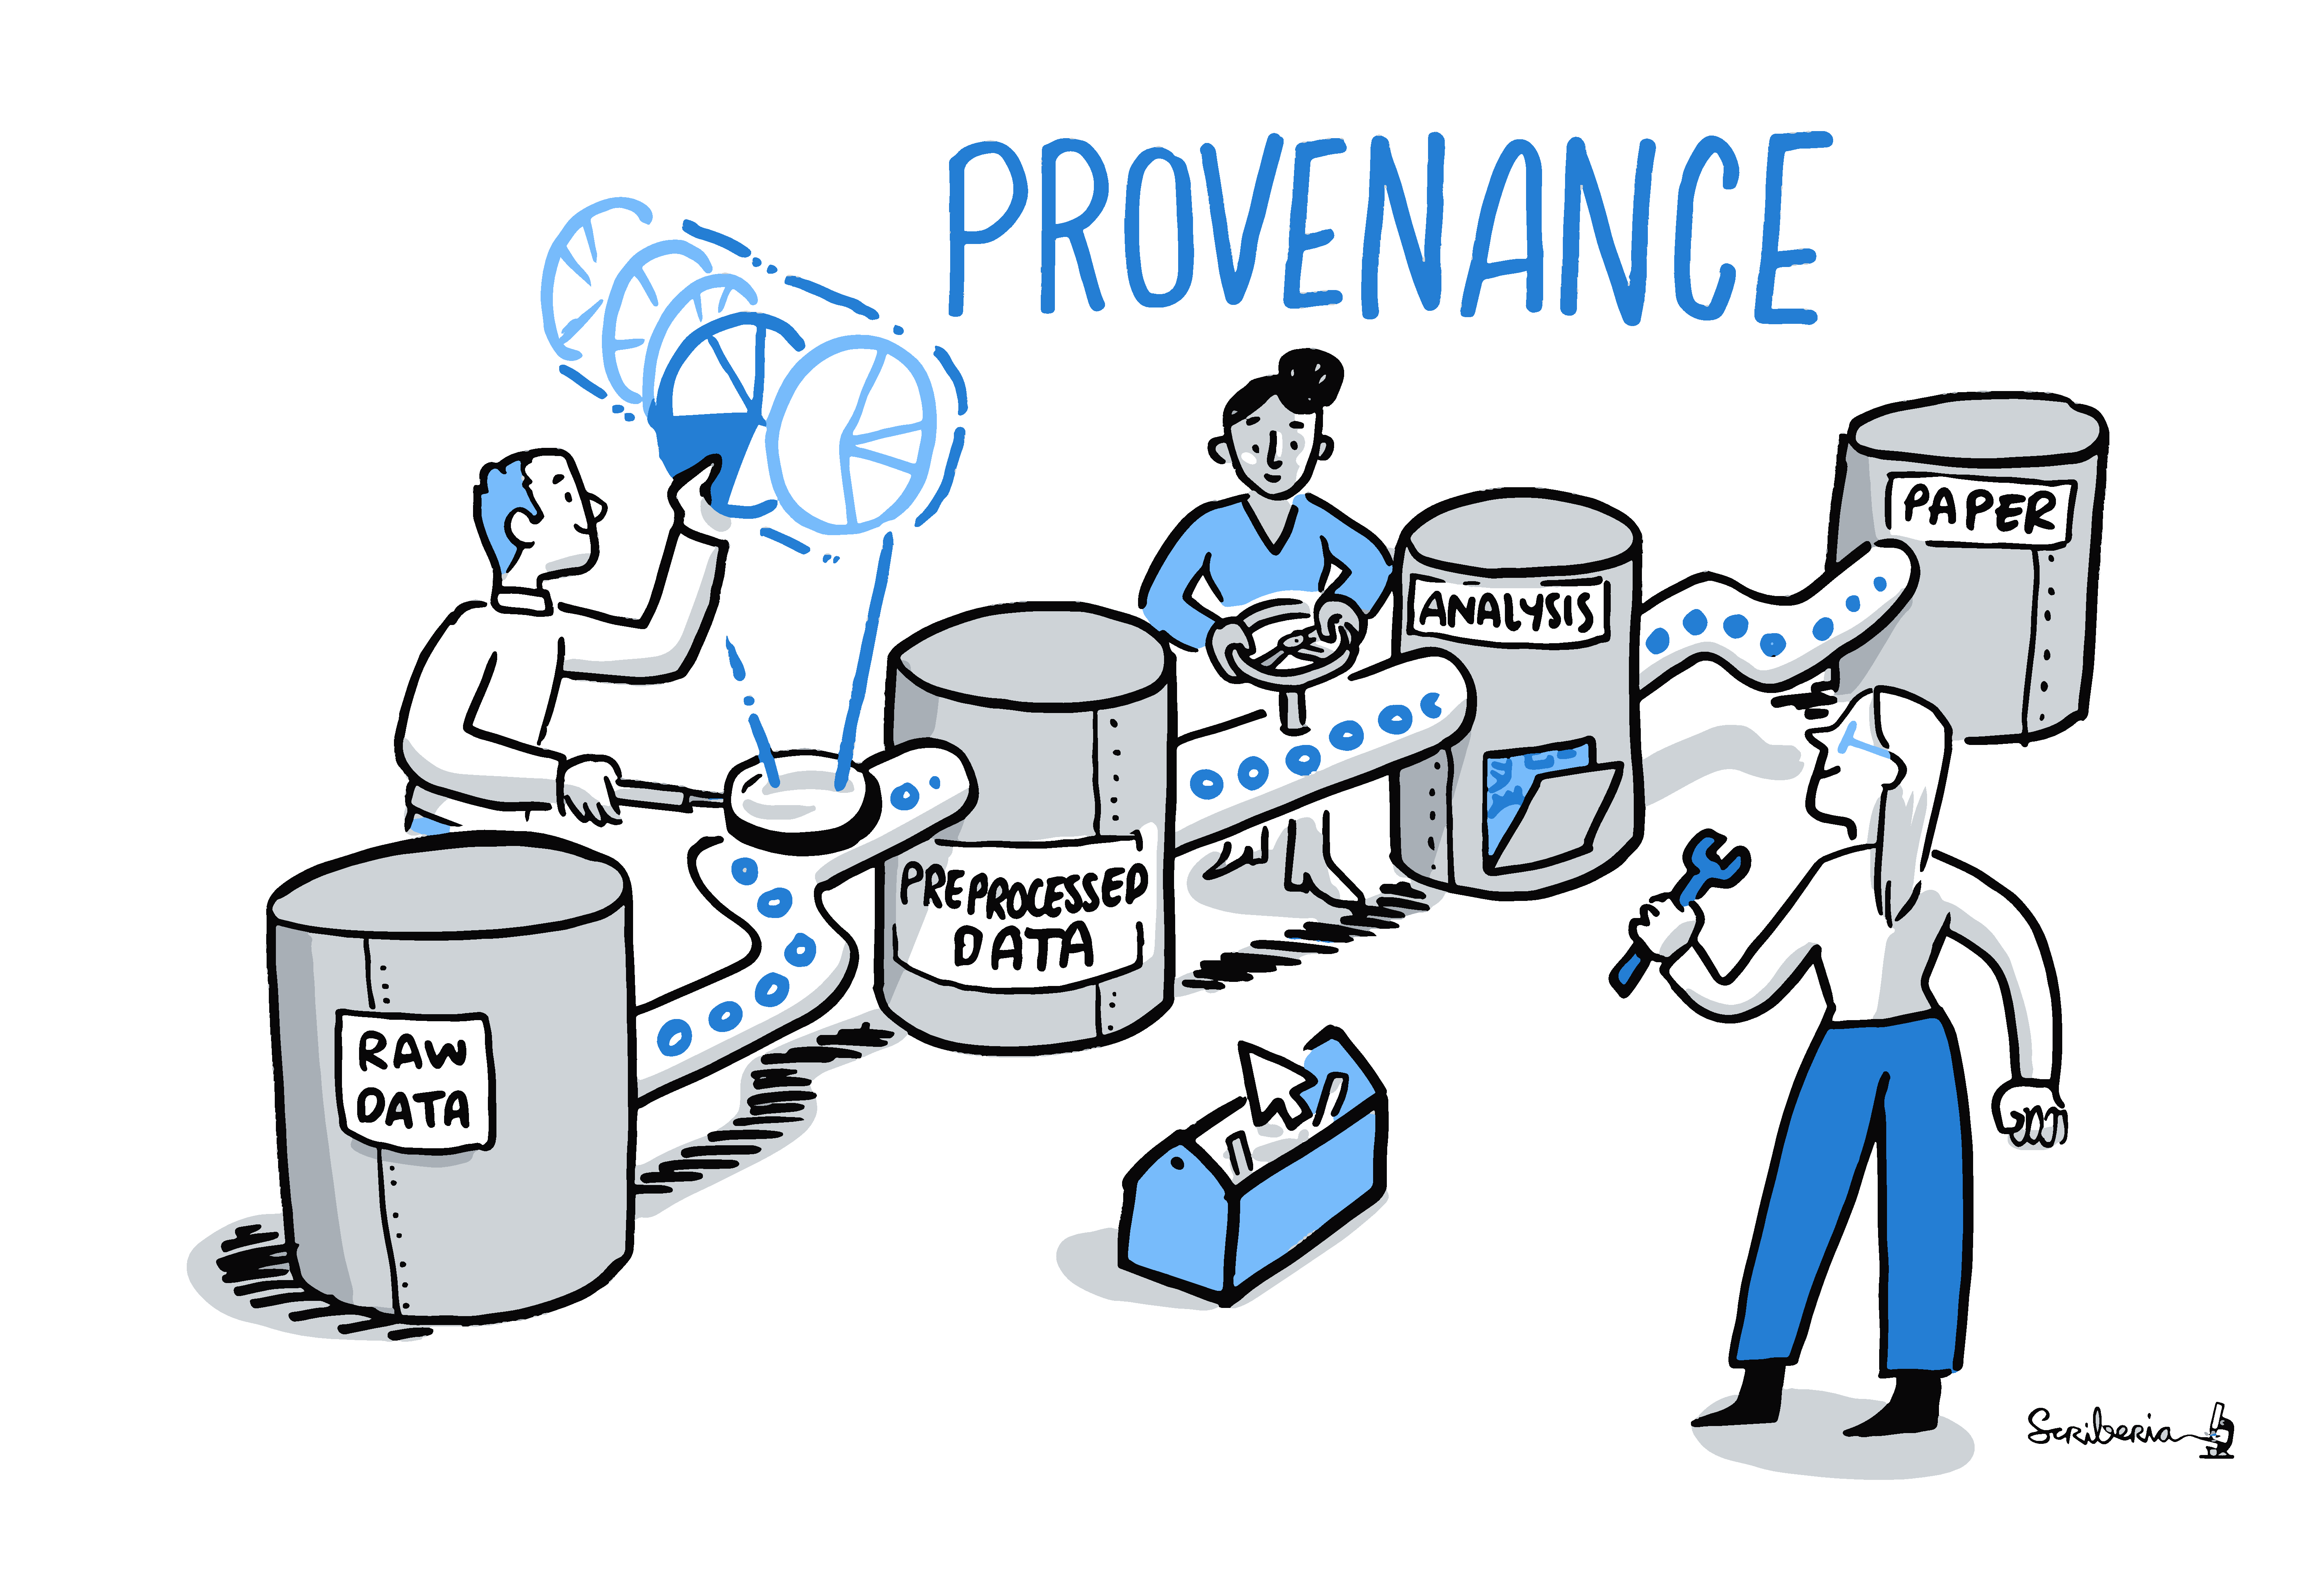
\includegraphics[width=.45\textwidth]{provenance.pdf}
	\caption[Provenance throughout the research process]{A variety of choices affect a research outcome. Digital provenance, information about how tools, data, and actors were involved in its generation, is required to retrace, understand, and trust the decisions that led to it. Good research data management yields good provenance. License: Scriberia and the Turing Way Project, CC-BY.}
	\label{fig:prov1}
\end{figure}



Overall, careful \gls{rdm} is necessary to translate complex data with difficult storage requirements and sophisticated processing workflows efficiently into scientific insights in the field of neuroimaging.
Given these specific complexities, solutions to these challenges often arise from the community of researchers.
The following section will highlight one of several software tools that aids with the complex task of research data management: DataLad.
%A subsequent chapter, \cref{chap:k2}, will later focus on how research data management is a prerequisite of reproducible research, specifically with regards to software environments and large sample sizes.
%In addition, \cref{chap:k2} will highlight pragmatic approaches to \gls{rdm} that can be embedded in standard research practice and contribute to the FAIRification of data, even in absence of established metadata formats.





% link to chapter 3: Research data management is a prerequisite of reproducible research

\section{DataLad as a software solution for research data management challenges}

%\[
%\left[
%\begin{tabular}{@{\quad}m{.3\textwidth}@{\qquad}m{.6\textwidth}@{\quad}}
%	\includegraphics[width=.7\linewidth]{qr_pub_datalad.png} &
%	\raggedright%
%	\textbf{Related publications} \par
	The following section provides an overview of the software tool DataLad and its use for research data management.
	The reader is invited to refer to our original publication \citep{Halchenko2021} for a more detailed description.%
%\end{tabular}
%\right]
%\]

%This introduces DataLad as a software solution for research data management

DataLad (\href{http://datalad.org}{datalad.org}) is a Python-based, MIT-licensed software tool for the joint management of code, data, and their relationship.
It builds up on git-annex, a versatile system for data logistics \citep{hessannex}, and Git, the industry standard for distributed version control.
To address the technical challenges of data management, data sharing, and digital provenance collection, it adapts principles of open-source software development and distribution to scientific workflows. \\
%Initially, DataLad development started with the idea to make data retrieval as easy as installing software with package managers on Unix-based operating systems\footnote{On a Debian system, a user can install thousands of software package with a single command such as \texttt{apt get install <package-name>}.}.
%Now, DataLad aims to make data management as easy as managing code \citep{Halchenko2021}.
DataLad's aim is ``to make data management as easy as managing code'' \citep{Halchenko2021}.
The latter benefits from a well-established ecosystem of tools, platforms, and processes.
The distributed version control tool Git provides the ability to track changes in small-sized, text-based files, and is a de-facto standard in collaborative software development. In 2022, 93.78\% of respondents in Stackoverflow's annual developer survey (\url{survey.stackoverflow.co}) reported to use it.
Hosting platforms for Git repositories such as GitHub (\url{github.com}), GitLab ({\url{gitlab.com}), or Gin (\url{gin.g-node.org}) have been developed to serve as facilitators for collaboration, discovery, and reuse.
In the scientific community it is widely recommended to employ version control for code to foster reproducibility \citep[e.g.,][]{sandve2013ten}, and it is established practice to develop and share research software and code using Git and Git hosting platforms \citep[e.g.,][]{nord2019towards, strupler2017reproducibility, bryan2018excuse, corti2019managing}.
But other components of scientific projects, such as data or computing environments, are not as transparently managed or accessible as code and software.
Digital research objects are usually stored in multiple different locations \citep{parsons2013research}, and their consumption is complicated by disconnected and non-interoperable hosting solutions:
Different storage services use different protocols, means of authentication, or other idiosyncrasies that require custom workflows.
Moreover, as will be elaborated in Chapter \ref{chap:k3}, scientific computation is not reproducible enough, because data provenance is often incomplete and rarely automatically captured.
And over the course of a research project, often as part of the standard, multi-stepped processing workflow, data evolve and change just like code does:
Continued acquisitions enlarge the raw dataset; Transformations to -- likewise evolving -- community standards change file formats, dataset organization, or enrich available metadata; And continuous quality control processes can fix errors in datasets.
In the case that data or other research objects were subject to change over the course of a project, there is a need to identify which exact version has been used -- otherwise, the reproducibility of a result is threatened \citep{hardwicke2018data}.
Yet unlike code in software development, data tend not to be as precisely identifiable because data versioning is rarely or only coarsely practiced.
Last but not least, in the absence of standardized data packages, there is no uniform way to declare actionable
data dependencies and derivative relationships between inputs and outputs of a computation.
Consequentially, data needs to be kept alongside to results to ensure reproducibility, even if it is hosted elsewhere already.
Especially in the age of big data neuroscience \citep{bzdok2017inference}, downloads or storage of datasets can become infeasible \citep{horien2021hitchhiker, grisham2016proposed}.
And although projects might only draw insights from only a subset of a dataset, such as only specific modalities, tasks, or participants, a project has heavier disk space demands if the original dataset is only available as a bulk download.\\
DataLad aims to solve these issues by providing streamlined, transparent management of code, data, computing environments, and their relationship.
Its main features are 1) Version control for data of any size or type; 2) Streamlined procedures to consume, publish, and update  all elements of scientific projects, with interoperability adapters to established scientific and commercial tools and services; 3) Data linkage as precisely versioned, lightweight dependencies; And 4) actionable process provenance capture for arbitrary command execution that affords automatic re-execution.

\subsection{Technical features}

Fundamental to DataLad's functionality is the concept of the ``DataLad dataset'', DataLad's central data structure.
On a technical level, it is a joint Git and git-annex repository with additional metadata and features for scientific use cases added on top by DataLad.\\
Git excels at managing and collaborating on text files, and provides a powerful backbone to DataLad's features.
Git repositories can be easily distributed as linked \textit{clones} to suitable infrastructure to share files and their revision history.
Locally, changes to files can be saved (\textit{committed}) with detailed provenance and transferred (\textit{pushed}) to all clones of a repository, and remote revisions can be retrieved and integrated (\textit{pulled}).\\
However, Git is not designed to handle large or binary files as common in science.
Git-annex overcomes this limitation and adds support to track and transfer files of arbitrary size or type without placing their content into Git.
Instead, it places file content into a managed repository \textit{annex} and only commits a lightweight reference that encodes the file's name and content identity via content hash into Git.
This reference allows a decoupling of file content (handled by git-annex) and filename (tracked with Git), but retains the ability to transparently notice and track changes: If file content changes, the identity reference known to Git changes, too, and the version control system becomes aware of the modification.
The same mechanism guarantees file integrity at all times and solves data privacy concerns without impacting discoverability, as potentially sensitive content can be kept private but its metadata can be distributed easily.
While Git keeps a reference of the content \textit{identity}, git-annex tracks content \textit{availability}, and manages data transport with an extensible set of protocols and set of hosting solutions to and from a local repository annex at a granularity of individual files. \\
DataLad, finally, extends Git and git-annex with easy to use modularization, re-executable annotation of changes, and targeted interfaces and interoperability adapters:
Modularization facilitates reusability in research workflows with large amount of files or with a heterogeneous nature, comprising different data sources or processing stages.
Organizing them into a modular structure of homogeneous or smaller components enables more efficient reuse.
DataLad allows to nest individual datasets via versioned linkage as lightweight dependencies, and provides seamless recursive operations across dataset boundaries by extending Git’s submodule mechanism.
With this, DataLad provides a ``monorepo''-like user experience in datasets with arbitrarily deep nesting, and makes it trivial to operate on individual files deep in the hierarchy or entire trees of datasets, while individual datasets can easily be reused in new contexts (see \cref{fig:subdslinkage}).\\
Re-executable annotations of changes constitute process provenance.
In DataLad datasets, DataLad can wrap any command execution and automatically capture the command, the generated outputs or modification, and optionally all required input elements with a so-called \texttt{datalad run} or a \texttt{datalad containers-run} command.
The former command captures the execution of any shell command, and the latter command can use software containers, tracked in DataLad datasets, for executing commands inside a specific software environment or containerized pipeline.
Both commands retrieve inputs, initiate command execution, and, if it succeeds, save results together with a re-executable provenance in a structured annotation to a Git commit message (see \cref{fig:fairly_metadata}).
In addition to providing reliable information about past command-line invocations, these machine-readable records make it possible to easily re-execute commands, for example to verify if a result is computationally reproducible or to apply an analog change to a different dataset state.\\
Interoperability adapters, finally, streamline data publication and consumption routines.
Being able to efficiently retrieve and update research objects across a variety of available storage options is an important part of \gls{rdm} \citep{borghi2018data}.
Git can already interact with other local or remote repositories via standard or custom network transport protocols, and git-annex readily provides access to a wide range of external data storage resources via a large set of protocols.
On top of this, DataLad implements support for additional services that require custom protocols, such as the \gls{osf} \citep{hanke2021dlosf}, and can add more fine-grained access (e.g. direct access to individual components contained in an archive hosted on cloud storage).
With this approach, DataLad can help to overcome technological limitations of storage solutions, or integrate seamlessly with technology that is already in use.

\begin{figure}
	\centering
	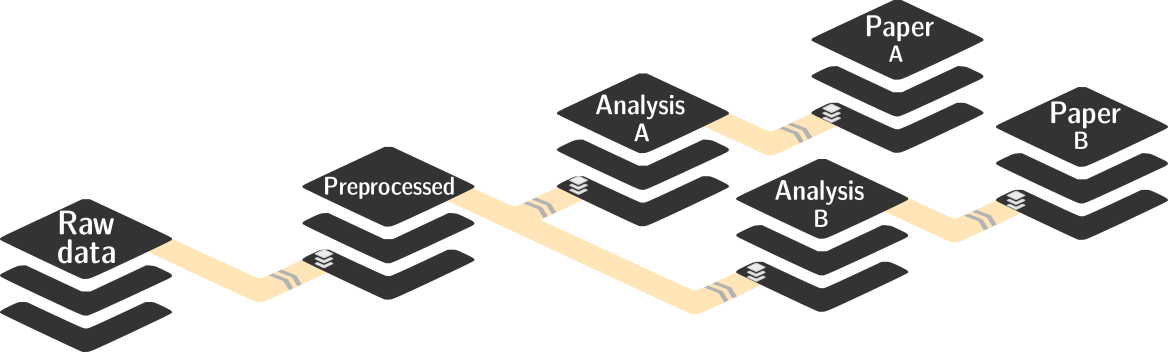
\includegraphics[width=.6\textwidth]{linkage_subds.png}
	\caption[DataLad dataset linkage]{Exemplary dataset hierarchy in a research project. DataLad datasets can be linked as actionable superdataset-subdataset relationships. A DataLad dataset with raw data is linked as a dependency to preprocessed data, to an analysis, and the final paper. As DataLad datasets decouple sizable file content from file availability metadata, such links are only a fraction of the size of the data they track. This feature enables modular projects from stand-alone units that facilitate reuse.}
	\label{fig:subdslinkage}
\end{figure}

\subsection{Development principles}

DataLad's development is guided by four principles \citep{Halchenko2021}:
\begin{itemize}
	\item The only two recognized entities are Datasets and the files they comprise,
	\item A dataset is a Git repository with an optional annex,
	\item The should be as few custom procedures and data structures as possible,
	\item Complete decentralization, with no required central server or service, but maximum interoperability with existing third-party resources and infrastructure.
\end{itemize}

These principles ensure DataLad's open and domain agnostic nature, maximize the long-term utility of DataLad datasets, minimize users' technical debt and reduce the risk of adoption.
When using DataLad datasets for digital objects, access to any resource managed with DataLad has no critical dependency on service deployments governed by central entities, and even on DataLad itself.
A further characteristic is that DataLad is developed not as a singular tool, but as an extensible ecosystem of software packages.
A core package provides basic functionality, and DataLad extensions, stand-alone Python packages with additional DataLad functionality, can enhance it with domain-focused or technology-specific features.
This aims to keep the source code maintainable, and allows users to tune the command-suite to their specific needs.


\subsection{User experience}

On the conceptual level, a DataLad dataset is an overlay structure to version control files of any size, track and publish files in a distributed fashion, and record, publish, and execute actionable provenance of files and file
transformations.
On a file system, it appears like a regular directory.
Users can either create DataLad datasets from scratch (\texttt{datalad create}) or install them from a variety of sources (\texttt{datalad clone}).
When consuming DataLad datasets from external sources, annexed file content can be retrieved (\texttt{datalad get}) and removed (\texttt{datalad drop}) on demand if the given user has potentially necessary access rights.
Generally, DataLad's commands aim to simplify standard workflows from Git, git-annex, or hosting services to make them more accessible to technical novices.
For example, committing a file into Git requires a \texttt{git add} followed by a \texttt{git commit}, and annexing a file requires a \texttt{git annex add} followed by a \texttt{git commit}.
A \texttt{datalad save}, on the other hand, performs either action, with automatic decision making whether the file is annexed or committed to Git.
Likewise, publishing a repository to hosting sites usually requires interactions in the hosting site's web interface, but DataLad provides a set of \texttt{create-sibling-<service>} commands that spare users the need to visit the hosting service.
And publication dependencies or automatic configurations can publish Git revision history and annexed file contents conjunctly, using \texttt{datalad push}.
Provenance capture can be achieved by wrapping command executions in either a \texttt{datalad run} or \texttt{datalad containers-run}\footnote{The \texttt{datalad containers-run} command is provided by the \texttt{datalad-container} extension package, available with standard Python package managers.} command, and they can be re-executed using \texttt{datalad rerun} (see \cref{fig:fairly_metadata}).
When working in hierarchies of datasets, any command's \texttt{--recursive} parameter applies it to downstream datasets.
Despite the fact that DataLad provides its own set of commands, compatibility with all Git and git-annex functionality is retained, and users are free to chose their workflows.
Like Git and git-annex, DataLad is primarily developed as a command line tool, but a \gls{gui} exists as well (see \cref{fig:gooey}).\\
With DataLad's streamlined data transport routines, users can utilize web sources, including major cloud storage providers, paths on local or remote computational infrastructure, or neuroscientific data registries such as OpenNeuro \citep{markiewicz2021openneuro} for file storage or collaboration.
At the same time, the separation of file content and file name makes a lean, meta-data based representation independent from actual data retrieval.
Thus, datasets of arbitrary scale can be cloned, exposing file names and revision history of all contained files, and provide actionable access to its content at a fraction of their total size.
And in order to expose datasets for easier access, users can publish DataLad datasets to common repository hosting infrastructure as access points to install data, without actually publishing data contents to these services.
These features aid with \gls{rdm} tasks in scientific projects, were used extensively in upcoming data analyses.
A thorough overview of features can be found in the software's documentation, which is elaborated on in Chapter \ref{chap:k2},  a comprehensive use case for reprodcubility is detailed in Chapter \ref{chap:k3}, and Chapter \ref{chap:k4} describes its use in brain-state analyses.

% provenance
\begin{figure}
	\centering
	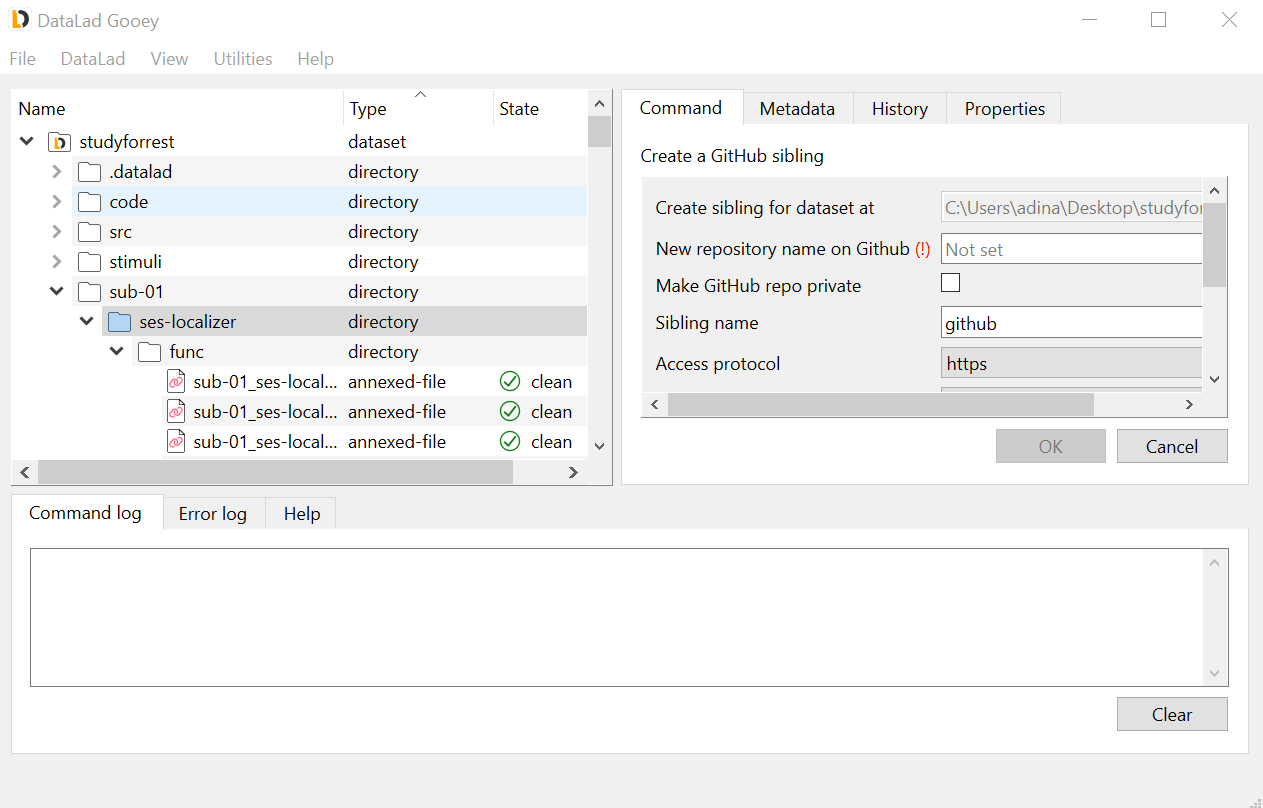
\includegraphics[width=.5\textwidth]{datalad_gooey.png}
	\caption[DataLad: Graphical User Interface]{The \gls{gui} provides an overview of working with DataLad. The file tree (left) is a DataLad dataset, and its contents are annotated whether they are tracked with Git, git-annex, or untracked, and whether they are modified, or if all changes are saved (``clean''). The command window (right) shows a DataLad command parametrization.}
	\label{fig:gooey}
\end{figure}

\subsection{Software adoption and relevance}

As DataLad does not employ tracking code, the exact number of its users is not known.
However, download statistics from the major Python package managers \texttt{pip} and \texttt{conda}, and popularity statistics from users of the Debian operating system can provide rough references.
According to \url{pypistats.org}, the main DataLad Python package was downloaded from the Python Package Index 474 times per day on average in August 2023.
The Python distribution Anaconda (\url{anaconda.org}) counts a total of 380.011 downloads of the software throughout versions 0.9.3 (April 2018) and 0.19.3 (August 2023), averaging 240 downloads per day.
The \texttt{popularity-contest} software is a Debian package that, if installed on a users system, reports anonymous statistics about most-used Debian packages.
This data is aggregated into a popularity contest.
According to it, in August 2023 between 0.08 and 0.12 percent of systems reporting statistics have a DataLad installation (see \cref{fig:popcon}), which is considerable when projected to the total amount of Debian-based computers world-wide.
All of these sources contain biases that limit conclusion to the number of users, though.
Installations via Python package managers are commonly performed by individual end users, whereas installations of Debian packages can correspond to system-wide installations on multi-user systems such as high performance computing infrastructure.
Likewise, upgrades of existing installations to more recent versions are included in these data, as well as temporary installations of the software in automated continuous integration test suites.
Nevertheless, download statistics attest that it is an actively used tool with a user base that exceeds the circle of its developers by far.
The citation count of our academic paper \citet{Halchenko2021}, totaling 66 in August 2023, and active contributor community around the source repository on GitHub, currently amounting to 48 individuals with committed code contributions, confirms that.
DataLad's current popularity, however, has not been established from the beginning of its development.
The next chapter will highlight how scientific software like DataLad can be improved and gain relevance, and, vice versa, improve scientific practice.
